\chapter{Un transmisor ISDBT implementado en GNU Radio}

\section{Generalidades del Transmisor}
Por ejemplo algunas
\section{El flujo de datos en GNU Radio}

\section{Obtencion de los TSP por capa}
\section{Codificaciones de Canal}
\section{La modulacion}
\section{El uso de los entrelazamientos}

\subsection{Entrelazamiento frecuencial}

El entrelazamiento frecuencial consiste en permutar las portadoras de un s\'imbolo OFDM en el dominio de la frecuencia. Dada la caracter\'istica de ISDB-T de utilizar un gran n\'umero de portadoras, ocurre que frente a canales selectivos en frecuencia se pueden ver afectadas una cantidad importante de portadoras consecutivas, con lo cual la capacidad de correcci\'on de los c\'odigos resultar\'ia superada.

Realizando un entrelazamiento frecuencial las portadoras que pudieran verse afectadas en un canal selectivo son desentrelazadas en recepci\'on y, por lo tanto, los errores que pudieran haber quedan distribu\'idos facilitando la tarea de los c\'odigos correctores.

El procedimiento del entrelazamiento en ISDB-T se divide en dos etapas: el \textit{enterlazamiento inter-segmentos}, y el \textit{entrelazamiento intra-segmentos }.

Primero se separan los segmentos en tres grupos: los destinados a recepci\'on parcial (\textit{one-seg}), los que utilizan \textit{modulaci\'on coherente}, y por otro lado los que utilizan \textit{modulaci\'ion diferencial}. Como en el caso de \textit{gr-isdbt-tx} s\'olo se utiliza modulaci\'on coherente, los caminos que pueden tomar los segmentos son \'unicamente dos.

Posteriormente viene la etapa de entrelazamiento inter-segmentos. Precisamente consiste en intercalar las portadoras entre los segmentos que comparten la modulac\'on. Para el segmento destinado a la recepci\'on parcial este proceso no tiene sentido, por lo cual pasa directamente a la etapa de enterlazamiento intra-segmento.

El entrelazamiento intra-segmento se realiza permutando las portadoras de cada segmento entre s\'i. Se comienza por rotar las portadoras de acuerdo a la siguiente expresi\'on:

Luego se realiza una aleatorizac\'on que est\'a determinada por \textit{Look Up Tables} que dependen del modo de transmisi\'on y puden consultarse en la referencia \cite{bb}.


\section{Entrelazamiento de bits}

Este bloque tiene a cargo esencialmente dos grandes tareas, primero entrelazar los bits que le ingresan provenientes de una determinada capa jerárquica dando lugar a un nuevo flujo de bits entrelazados. Luego estos bits son agrupados para formar símbolos complejos según la modulación que tenga la capa.

El proceso de entrelazamiento se lleva a cabo aplicando retardos definidos según la modulación. Esto supone utilizar una estructura de colas paralelas FIFO de distinto tamaño en las cuales se va colocando de a un bit a la vez. Una vez que se coloca un bit en cada cola, en el otro extremo se forma un complejo extrayendo el último bit de cada cola.

Inicialmente cuando se enciende el sistema se tendrá un transitorio con datos inválidos como producto del contenido de las colas previo al momento de que se inicializa el sistema. Esto no es inconveniente puesto que el receptor descarta esos datos y se sincroniza en un comienzo de frame válido.

Entrelazar utilizando esta mecanismo de colas de retardos variables implica agregar un retardo total correspondiente al camino más largo que deben atravesar los bits, es decir un retardo de 120 símbolos complejos. Según la modulación que utilice la capa estos 120 símbolos se traducen en un mayor o menor retardo en el tiempo; para QPSK corresponde a esperar que ingresen $120 \times 2$ bits en la entrada, mientras que para 64QAM deben pasar $120 \times 6$ bits.

Con el objetivo de tener un mismo retardo para lograr sincronismo en todas las capas se realiza un \textit{ajuste de atraso}. En ISDB-T los retardos deben ser m\'ultiplos de un s\'imbolo OFDM; para el entrelazamiento de bits el retardo propio del proceso de entrelazamiento sumado al ajuste de atraso debe totalizar dos s\'imbolos OFDM.

El tamano de un s\'imbolo OFDM corresponde a: 
\begin{equation}
N_{OFDM} = m_L \times N_L \times 96 \times 2^{modo-1} \quad \text{bits}
\end{equation}

$N_{OFDM}$ depende de la modulaci\'on de la capa $m_L$, que puede ser 2, 4 y 6 para QPSK, 16QAM y 64QAM respectivamente; la cantidad de segmentos utilizados $N_L$ y por supuesto del modo de transmisi\'on. La soluci\'on implementada en \textit{gr-isdbt-tx} consiste en incrementar los tamanos de las colas de manera que el retardo total sea de dos s\'imbolos OFDM para cada capa. Por lo tanto para tener el retardo deseado los tamanos de las colas deben ser:

\begin{equation}
Q_i = q_i + \dfrac{2 \times N_{OFDM} - 120 \times m_L}{m_L} = q_i + N_L \times 96 \times 2^{modo-1} - 120
\end{equation}

\begin{figure}[!h]
\centering
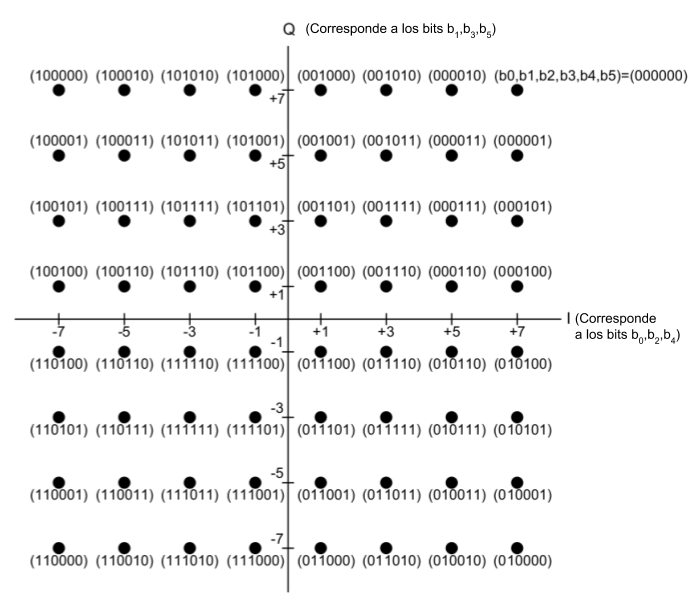
\includegraphics[scale=0.5]{figuras/cap05/constelacion_64QAM}
\caption{\label{f:mapeo_64QAM} Mapeo de la constelaci\'on 64QAM.}
\end{figure}

Una vez que son empujados los bits en cada cola, desde el otro extremo se extrae un bit por cola y se mapean en un s\'imbolo complejo de acuerdo a como lo establece la norma. Por ejemplo en la Figura \ref{f:mapeo_64QAM} se muestra c\'omo se realiza este mapeo para la modulaci\'on 64QAM. Por \'ultimo los complejos deben ser normalizados seg\'un un factor de normalizaci\'on que se presenta en la Tabla \ref{t:factor_normalizacion}.

\begin{table}[h!]
\centering
\begin{tabular}{|c|c|}
\hline
\textbf{Modulaci\'on} 				& \textbf{Factor de normalizaci\'on}\\
\hline
QPSK 		& $1/ \sqrt{2}$\\
\hline
16QAM		& $1/ \sqrt{10}$ \\
\hline
64QAM 		& $1/ \sqrt{42}$ \\
\hline
\end{tabular}
\caption{\label{t:factor_normalizacion} Factores de normalizaci\'on para los distintos esquemas de modulaci\'on.}
\end{table}


\section{Entrelazamiento temporal}

El entrelazamiento temporal consiste en distribu\'uir los s\'imbolos complejos entre distintos s\'imbolos OFDM. Esta distribuci\'on o entrelazamiento se realiza para cada portadora, es decir que se realiza en el dominio del tiempo.

Esta t\'ecnica act\'ua como mecanismo de protecci\'on frente a ruidos impulsivos que t\'ipicamente se caracterizan por una corta duraci\'on en el tiempo. La profundidad o largo del entrelazamiento temporal es el par\'ametro que rige este proceso de entrelazado y puede ser seteado de manera independiente para cada capa. Est\'a \'intimamente ligado a la dispersi\'on temporal que se realiza en los s\'imbolos; a mayor profundidad, los s\'imbolos de una misma portadora son retardados un tiempo mayor.

La Figura \ref{f:entrelazamiento_temporal} describe esquem\'aticamente el mecanismo de entrelazamiento. Consiste en aplicar un retardo distinto para cada s\'imbolo dentro de un mismo segmento; los segmentos de una misma capa son retardados de igual manera seg\'un la profundidad de entrelazamiento elegida. 

La implementaci\'on de estos retardos en \textit{gr-isdbt-tx} es llevada a cabo por medio de colas en las que, de manera secuencial, se empujan los s\'imbolos que van arribando correspondientes a las distintas capas jer\'arquicas. Desde el otro extremo se extrae un s\'imbolo de cada cola tambi\'en de manera secuencial. 

Para una capa jer\'arquica con profundidad de entrelazamiento $I_L$, los retardos estipulados por ISDB-T para cada uno de sus segmentos se define de la siguiente manera:

\begin{equation}
q_L(i) = I_L \times m_i = I_L \times ((i \times 5) \; mod \; 96)
\end{equation}

Donde $q_L(i)$ representa el tamano de las colas o búfers; $m_i$ es definido por el est\'andar como $m_i = (i \times 5) \; mod \; 96$, para $i = 0, 1,..,n_c$ con $n_c = 1$, $2$, o $3$ seg\'un el modo de transmisi\'on. 

\begin{figure}[!h]
\centering
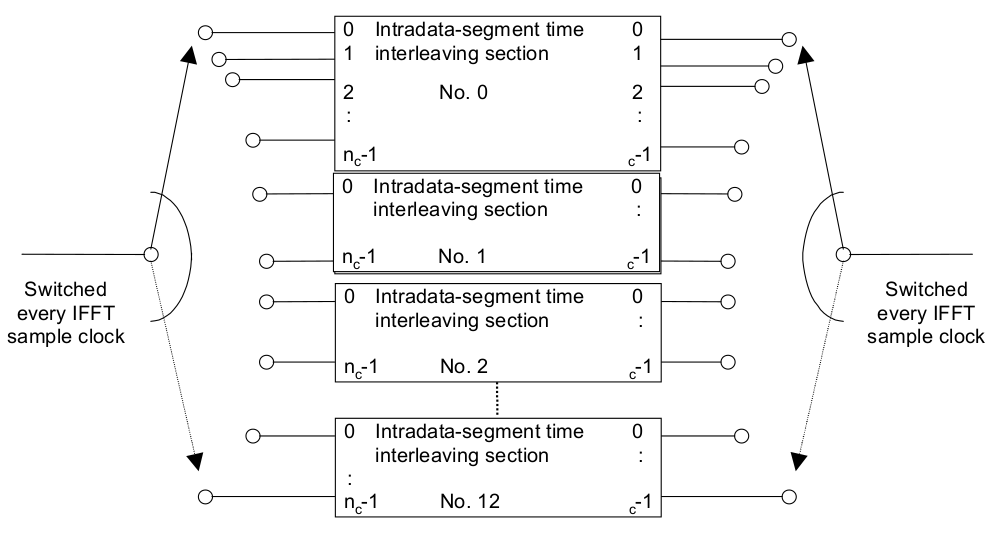
\includegraphics[scale=0.4]{figuras/cap05/entrelazamiento_temporal}
\caption{\label{f:entrelazamiento_temporal} Mecanismo de entrelazamiento temporal.}
\end{figure}



\section{Formacion de cuadros OFDM}
El cuadro OFDM es una estructura de datos que agrupa los datos de carga \'util, portadoras piloto y senales de control. Tiene todo lo necesario para que un receptor compatible con ISDB-T sea capaz de decodificarlo en flujos MPEG y reproducir la informaci\'on.

Se trata de un conjunto de 204 s\'imbolos OFDM, cada uno de ellos conformado por $13 \times 108 \times 2^{modo -1}$ s\'imbolos complejos. 







	\subsection{Las portadoras piloto}
	\subsection{Las portadoras activas}
\section{El prefijo ciclico}
\section{La transmision desde USRP}